\documentclass[12pt, twoside]{article}
\usepackage[letterpaper, margin=1in, headsep=0.5in]{geometry}
\usepackage[english]{babel}
\usepackage[utf8]{inputenc}
\usepackage{amsmath}
\usepackage{amsfonts}
\usepackage{amssymb}
\usepackage{tikz}
\usepackage{yhmath}
%\usetikzlibrary{quotes, angles}

\usepackage{graphicx}
\usepackage{enumitem}
\usepackage{multicol}

\usepackage{fancyhdr}
\pagestyle{fancy}
\fancyhf{}
\renewcommand{\headrulewidth}{0pt} % disable the underline of the header

\fancyhead[RE]{\thepage}
\fancyhead[RO]{\thepage \\ Name: \hspace{3cm}}
\fancyhead[L]{BECA / Dr. Huson / 10th Grade Geometry\\* 22 May 2019}

\begin{document}
\subsubsection*{11.3 Do Now: Quadrilaterals}
 \begin{enumerate}

   \item Given rhombus $ABCD$ with $m\angle A=45^\circ$, and $AB=7$. Find the value of each angle measure or side length.
   \begin{multicols}{2}
     \begin{enumerate}
       \item $m\angle B=$\vspace{0.5cm}
       \item $m\angle C=$\vspace{0.5cm}
       \item $m\angle D=$\vspace{0.5cm}
       \item $CD=$ \vspace{0.5cm}
       \item $AD=$ \vspace{0.5cm}
     \end{enumerate}
     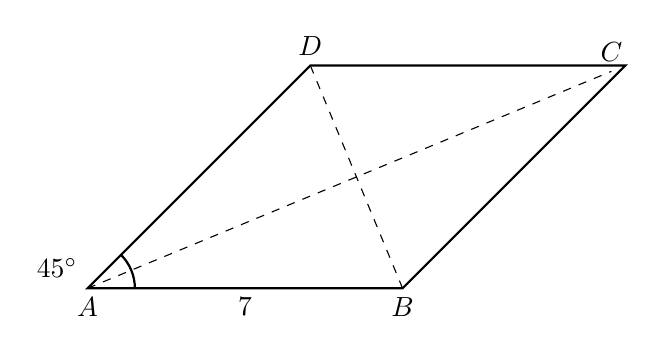
\begin{tikzpicture}[scale=.8]
       \draw [thick] (0,0)node[above left]{$45^\circ$}--(5,0)--++(45:5)--(45:5)--cycle;
       \draw [thick] (0.75,0) arc [start angle=0, end angle=45, radius=0.75];
       \draw [dashed] (0,0)node[below]{$A$}--(22.5:9)node[above]{$C$};
       \draw [dashed] (5,0)node[below]{$B$}--(45:5)node[above]{$D$};
       \node at (2.5,0)[below]{$7$};
     \end{tikzpicture}
   \end{multicols}

  \item Circle Always, Sometimes, Never, as applies.
  \begin{center}
    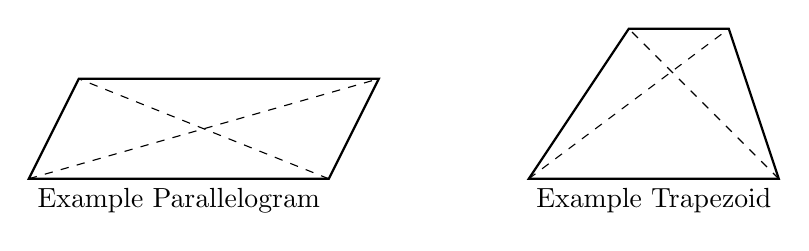
\begin{tikzpicture}[scale=.635]
      \draw [thick] (-2,0) -- (4,0)--(5,2)--(-1,2)--cycle;
      \draw [dashed] (-2,0)--(5,2);
      \draw [dashed] (4,0)--(-1,2);
      \node at (1,0)[below]{Example Parallelogram};

      \draw [thick] (8,0) -- (13,0)--(12,3)--(10,3)--cycle;
      \draw [dashed] (8,0)--(12,3);
      \draw [dashed] (13,0)--(10,3);
      \node at (10.5,0)[below]{Example Trapezoid};
    \end{tikzpicture}
  \end{center}
    \begin{enumerate}
      \item Always \quad Sometimes \quad  Never \quad Opposite sides of a parallelogram are parallel. \vspace{0.25cm}
      \item Always \quad Sometimes \quad  Never \quad Diagonals of a parallelogram are congruent. \vspace{0.25cm}
      \item Always \quad Sometimes \quad  Never \quad One pair of opposite sides of a trapezoid are parallel. \vspace{0.25cm}
      \item Always \quad Sometimes \quad  Never \quad Opposite angles of a rhombus are congruent.
    \end{enumerate}

  \item The long diagonal of rhombus PQRS measures $PR=8$ and the short diagonal is $QS=6$. The intersection of the diagonals is $M$. Find the given measures.\vspace{0.25cm}
    \begin{multicols}{2}
      \begin{enumerate}
        \item $PM=$ \vspace{0.5cm}
        \item $QM=$ \vspace{0.5cm}
        \item $PQ=$ \vspace{0.5cm}
        \item $m\angle SPQ=$\vspace{1.5cm}
      \end{enumerate}
      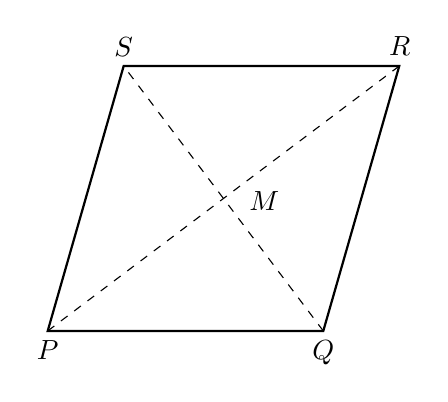
\begin{tikzpicture}[scale=.7]
        \draw [thick] (0,0)--(5,0)--++(74:5)--(74:5)--cycle;
        \draw [dashed] (0,0)node[below]{$P$}--(37:8)node[above]{$R$};
        \draw [dashed] (5,0)node[below]{$Q$}--(74:5)node[above]{$S$};
        \node at (34:4.2)[right]{$M$};
      \end{tikzpicture}
    \end{multicols}

\end{enumerate}
\end{document}
